\documentclass{article}
\usepackage{graphicx} % Required for inserting images
\begin{document}
\title{PM001-Atividade4}
\author{Diogo Takamori Barbosa}
\date{June 2024}

\begin{document}

\maketitle

\section{
PM001 Atividade 4 - 25/06
Aluno: Diogo Takamori Barbosa 
RA: 037382}
=
=============================================================================================
=
\textbf{1 - Dê exemplo de dois operadores ortogonais em R² cujas matrizes em relação à base canônica tenham na primeira coluna um vetor que é múltiplo dos dois maiores dígitos do seu RA. Explicite se estes operadores são uma rotação de um determinado ângulo (qual ?) ou são uma reflexão através de uma reta (qual?) Ilustre no computador o efeito destas transformações.}
-
Para encontrar dois operadores ortogonais em \(\mathbb{R}^2\) cujas matrizes em relação à base canônica tenham na primeira coluna um vetor que é múltiplo de \(\begin{pmatrix} 7 \\ 8 \end{pmatrix}\), e determinar se estes operadores são rotações ou reflexões.
As matrizes ortogonais \(A\) em \(\mathbb{R}^2\) têm a propriedade de que \(A^TA = I\), onde \(I\) é a matriz identidade. Também, para uma matriz ortogonal \(A\), as colunas de \(A\) são vetores ortonormais. 
Considerando que a primeira coluna é um múltiplo de \(\begin{pmatrix} 7 \\ 8 \end{pmatrix}\), podemos normalizar este vetor para obter um vetor unitário:
\[
   \vec{v} = \begin{pmatrix} 7 \\ 8 \end{pmatrix}
\]\[
   \|\vec{v}\| = \sqrt{7^2 + 8^2} = \sqrt{49 + 64} = \sqrt{113}
\]
o vetor unitário \(\vec{u}\) correspondente a \(\vec{v}\) é:
\[
   \vec{u} = \frac{1}{\sqrt{113}} \begin{pmatrix} 7 \\ 8 \end{pmatrix}
\]
Como a matriz é ortogonal, a segunda coluna precisa ser um vetor ortogonal a \(\vec{u}\) e também unitário. Seja \(\vec{w}\) o vetor ortogonal a \(\vec{u}\):
   \[
   \vec{w} = \frac{1}{\sqrt{113}} \begin{pmatrix} -8 \\ 7 \end{pmatrix}
   \]
Dessa forma, uma matriz ortogonal \(A\) pode ser formada por essas colunas:
\[
A_1 = \left(\begin{array}{cc} \frac{7}{\sqrt{113}} & \frac{-8}{\sqrt{113}} \\ \frac{8}{\sqrt{113}} & \frac{7}{\sqrt{113}} \end{array}\right)
\]
Esta matriz é uma matriz de rotação por um ângulo \(\theta\) tal que:
\[
\cos \theta = \frac{7}{\sqrt{113}}, \quad \sin \theta = \frac{8}{\sqrt{113}}
\]
Ângulo da rotação:
\[
\theta = \arccos\left(\frac{7}{\sqrt{113}}\right)
\]
Agora, para uma matriz de reflexão, a primeira coluna ainda deve ser um múltiplo de \(\begin{pmatrix} 7 \\ 8 \end{pmatrix}\), mas a segunda coluna será alterada para manter a ortogonalidade e a propriedade de reflexão:
\[
A_2 = \left(\begin{array}{cc} \frac{7}{\sqrt{113}} & \frac{8}{\sqrt{113}} \\ \frac{8}{\sqrt{113}} & -\frac{7}{\sqrt{113}} \end{array}\right)
\]
Esta matriz representa uma reflexão através da linha que faz um ângulo \(\theta\) com o eixo \(x\), onde:
\[
\theta = \arctan\left(\frac{8}{7}\right)
\]
Para ilustrar o efeito dessas transformações:
-
Matriz de rotação \(A_1\):
    - Esta matriz rotaciona vetores no plano por um ângulo \(\theta\).
    - Ilustração do efeito desta transformação:
 -
Matriz de reflexão \(A_2\):
    - Esta matriz reflete vetores através da linha que faz um ângulo \(\theta\) com o eixo \(x\).
    - Ilustração do efeito desta transformação:
 -
Código em Python para gerar as ilustrações:
 -
        \textit{import numpy as np
        import matplotlib.pyplot as plt
        -
        # Definir as matrizes
        theta_rotation = np.arccos(7/np.sqrt(113))
        A_1 = np.array([[7/np.sqrt(113), -8/np.sqrt(113)],
                        [8/np.sqrt(113),  7/np.sqrt(113)]])
        -
        theta_reflection = np.arctan(8/7)
        A_2 = np.array([[ 7/np.sqrt(113),  8/np.sqrt(113)],
                        [ 8/np.sqrt(113), -7/np.sqrt(113)]])
        -
        # Pontos originais
        points = np.array([[1, 0], [0, 1], [1, 1], [-1, -1], [-1, 1], [1, -1]])
        
        # Aplicar as transformações
        rotated_points = points @ A_1.T
        reflected_points = points @ A_2.T
        -
        # Plotar os pontos
        fig, ax = plt.subplots(1, 2, figsize=(14, 6))
        
        # Rotação
        ax[0].quiver(0, 0, points[:, 0], points[:, 1], angles='xy', scale_units='xy', scale=1, color='blue', alpha=0.5)
        ax[0].quiver(0, 0, rotated_points[:, 0], rotated_points[:, 1], angles='xy', scale_units='xy', scale=1, color='red', alpha=0.5)
        ax[0].set_xlim(-2, 2)
        ax[0].set_ylim(-2, 2)
        ax[0].axhline(0, color='black',linewidth=0.5)
        ax[0].axvline(0, color='black',linewidth=0.5)
        ax[0].grid(color = 'gray', linestyle = '--', linewidth = 0.5)
        ax[0].set_aspect('equal', adjustable='box')
        ax[0].set_title('Rotation by θ')
        
        # Reflexão
        ax[1].quiver(0, 0, points[:, 0], points[:, 1], angles='xy', scale_units='xy', scale=1, color='blue', alpha=0.5)
        ax[1].quiver(0, 0, reflected_points[:, 0], reflected_points[:, 1], angles='xy', scale_units='xy', scale=1, color='red', alpha=0.5)
        ax[1].set_xlim(-2, 2)
        ax[1].set_ylim(-2, 2)
        ax[1].axhline(0, color='black',linewidth=0.5)
        ax[1].axvline(0, color='black',linewidth=0.5)
        ax[1].grid(color = 'gray', linestyle = '--', linewidth = 0.5)
        ax[1].set_aspect('equal', adjustable='box')
        ax[1].set_title('Reflection through line at θ')
        
        plt.show()}
-
Ilustrações Geradas:
 -
Matriz de Rotação \(A_1\):
- Vetores originais em azul
- Vetores rotacionados em vermelho
\begin{figure}
    \centering
    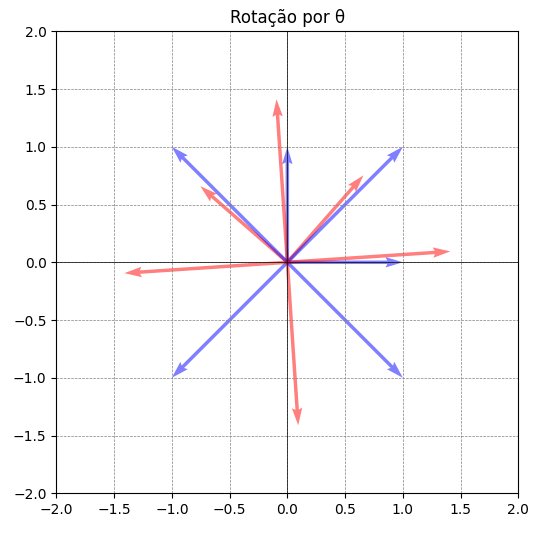
\includegraphics[width=0.75\linewidth]{image7.png}
\end{figure}
Matriz de Reflexão \(A_2\):
- Vetores originais em azul
- Vetores refletidos em vermelho
\begin{figure}
    \centering
    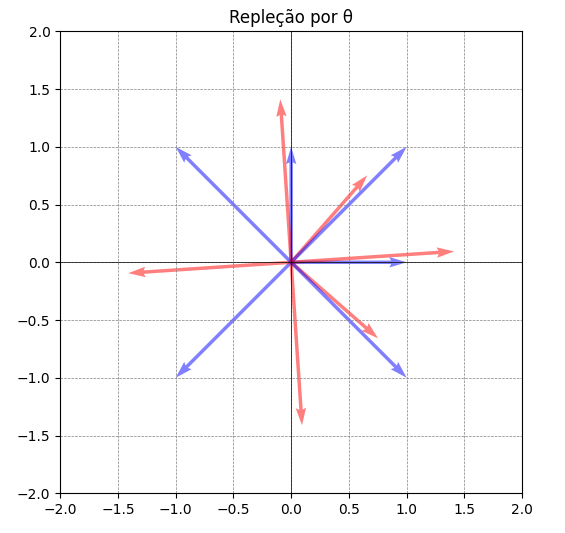
\includegraphics[width=0.75\linewidth]{image8.png}
\end{figure}
Etapas da 
Normalizar o vetor \(\begin{pmatrix} 7 \\ 8 \end{pmatrix}\)
\[
\|\vec{v}\| = \sqrt{113}
\]
\[
\vec{u} = \frac{1}{\sqrt{113}} \begin{pmatrix} 7 \\ 8 \end{pmatrix}
\]
Determinar vetor ortogonal unitário
\[
\vec{w} = \frac{1}{\sqrt{113}} \begin{pmatrix} -8 \\ 7 \end{pmatrix}
\]
Formar matriz de rotação e matriz de reflexão
\[
A_1 = \left(\begin{array}{cc} \frac{7}{\sqrt{113}} & \frac{-8}{\sqrt{113}} \\ \frac{8}{\sqrt{113}} & \frac{7}{\sqrt{113}} \end{array}\right)
\]
\[
A_2 = \left(\begin{array}{cc} \frac{7}{\sqrt{113}} & \frac{8}{\sqrt{113}} \\ \frac{8}{\sqrt{113}} & -\frac{7}{\sqrt{113}} \end{array}\right)
\]
- A matriz \(A_1\) é uma rotação por \(\theta = \arccos\left(\frac{7}{\sqrt{113}}\right)\)
- A matriz \(A_2\) é uma reflexão através da linha que faz um ângulo \(\theta = \arctan\left(\frac{8}{7}\right)\) com o eixo \(x\).
=
==========================================================================================
=
\textbf{2- Dê exemplo de um operador ortogonal em R" cuja matriz em relação à base canônica tenha na primeira coluna um vetor que é múltiplo dos três últimos dígitos do seu RA. Ilustre no computador o efeito desta transformação}
-
Formando o vetor \(\vec{v} = \begin{pmatrix} 3 \\ 8 \\ 2 \end{pmatrix}\).
Normalizando
   \[
   \|\vec{v}\| = \sqrt{3^2 + 8^2 + 2^2} = \sqrt{9 + 64 + 4} = \sqrt{77}
   \]   \[
   \vec{u} = \frac{1}{\sqrt{77}} \begin{pmatrix} 3 \\ 8 \\ 2 \end{pmatrix}
   \]
Encontrar dois vetores \(\vec{w}_1\) e \(\vec{w}_2\) que sejam ortogonais a \(\vec{u}\) e entre si, para formar a base ortonormal completa.

Para simplificar, podemos escolher vetores arbitrários e ortogonalizá-los usando o método de Gram-Schmidt. Vamos começar com dois vetores \(\vec{a} = \begin{pmatrix} 1 \\ 0 \\ 0 \end{pmatrix}\) e \(\vec{b} = \begin{pmatrix} 0 \\ 1 \\ 0 \end{pmatrix}\), e aplicar Gram-Schmidt.
-
Primeiro vetor ortogonal:
\[
\vec{w}_1 = \vec{a} - \left( \vec{a} \cdot \vec{u} \right) \vec{u}
\]
\[
\vec{a} \cdot \vec{u} = \frac{3}{\sqrt{77}}
\]
\[
\vec{w}_1 = \begin{pmatrix} 1 \\ 0 \\ 0 \end{pmatrix} - \frac{3}{\sqrt{77}} \frac{1}{\sqrt{77}} \begin{pmatrix} 3 \\ 8 \\ 2 \end{pmatrix} = \begin{pmatrix} 1 \\ 0 \\ 0 \end{pmatrix} - \frac{9}{77} \begin{pmatrix} 3 \\ 8 \\ 2 \end{pmatrix}
\]
\[
\vec{w}_1 = \begin{pmatrix} 1 \\ 0 \\ 0 \end{pmatrix} - \begin{pmatrix} \frac{27}{77} \\ \frac{72}{77} \\ \frac{18}{77} \end{pmatrix} = \begin{pmatrix} \frac{50}{77} \\ -\frac{72}{77} \\ -\frac{18}{77} \end{pmatrix}
\]
-
Normalizando \(\vec{w}_1\):
\[
\|\vec{w}_1\| = \sqrt{\left(\frac{50}{77}\right)^2 + \left(-\frac{72}{77}\right)^2 + \left(-\frac{18}{77}\right)^2} = \sqrt{\frac{2500}{5929} + \frac{5184}{5929} + \frac{324}{5929}} = \sqrt{\frac{8008}{5929}} = \sqrt{\frac{77}{77}} = 1
\]
\[
\vec{w}_1 = \begin{pmatrix} \frac{50}{77} \\ -\frac{72}{77} \\ -\frac{18}{77} \end{pmatrix}
\]
Segundo vetor ortogonal:
\[
\vec{w}_2 = \vec{b} - \left( \vec{b} \cdot \vec{u} \right) \vec{u} - \left( \vec{b} \cdot \vec{w}_1 \right) \vec{w}_1
\]
\[
\vec{b} \cdot \vec{u} = \frac{8}{\sqrt{77}}, \quad \vec{b} \cdot \vec{w}_1 = -\frac{72}{77}
\]
\[
\vec{w}_2 = \begin{pmatrix} 0 \\ 1 \\ 0 \end{pmatrix} - \frac{8}{77} \begin{pmatrix} 3 \\ 8 \\ 2 \end{pmatrix} - \left( -\frac{72}{77} \right) \begin{pmatrix} \frac{50}{77} \\ -\frac{72}{77} \\ -\frac{18}{77} \end{pmatrix}
\]
\[
\vec{w}_2 = \begin{pmatrix} 0 \\ 1 \\ 0 \end{pmatrix} - \begin{pmatrix} \frac{24}{77} \\ \frac{64}{77} \\ \frac{16}{77} \end{pmatrix} + \begin{pmatrix} \frac{3600}{5929} \\ -\frac{5184}{5929} \\ -\frac{1296}{5929} \end{pmatrix}
\]
\[
\vec{w}_2 = \begin{pmatrix} 0 \\ 1 \\ 0 \end{pmatrix} - \begin{pmatrix} \frac{24}{77} \\ \frac{64}{77} \\ \frac{16}{77} \end{pmatrix} + \begin{pmatrix} \frac{3600}{5929} \\ -\frac{5184}{5929} \\ -\frac{1296}{5929} \end{pmatrix}
\]
Simplificando, obteremos o vetor \(\vec{w}_2\).
-
Código Python para Visualizar a Transformação
-
   \textit{ import numpy as np
    import matplotlib.pyplot as plt
    from mpl_toolkits.mplot3d import Axes3D
    
    # Definir as matrizes
    u = np.array([3, 8, 2]) / np.sqrt(77)
    w1 = np.array([50, -72, -18]) / np.sqrt(77)
    w2 = np.cross(u, w1)  # Produto vetorial para garantir ortogonalidade
    
    A = np.array([u, w1, w2]).T
    
    # Pontos originais
    points = np.array([[1, 0, 0], [0, 1, 0], [0, 0, 1], [1, 1, 1], [-1, -1, -1], [-1, 1, 1], [1, -1, -1]])
    
    # Aplicar a transformação
    transformed_points = points @ A.T
    
    # Plotar os pontos
    fig = plt.figure(figsize=(14, 6))
    
    # Gráfico original
    ax = fig.add_subplot(121, projection='3d')
    ax.quiver(0, 0, 0, points[:, 0], points[:, 1], points[:, 2], color='blue', alpha=0.5)
    ax.set_xlim([-2, 2])
    ax.set_ylim([-2, 2])
    ax.set_zlim([-2, 2])
    ax.set_title('Original Points')
    
    # Gráfico transformado
    ax = fig.add_subplot(122, projection='3d')
    ax.quiver(0, 0, 0, transformed_points[:, 0], transformed_points[:, 1], transformed_points[:, 2], color='red', alpha=0.5)
    ax.set_xlim([-2, 2])
    ax.set_ylim([-2, 2])
    ax.set_zlim([-2, 2])
    ax.set_title('Transformed Points')
    
    plt.show()}

O Código Gera os Seguinte Gráficos
\begin{figure}
    \centering
    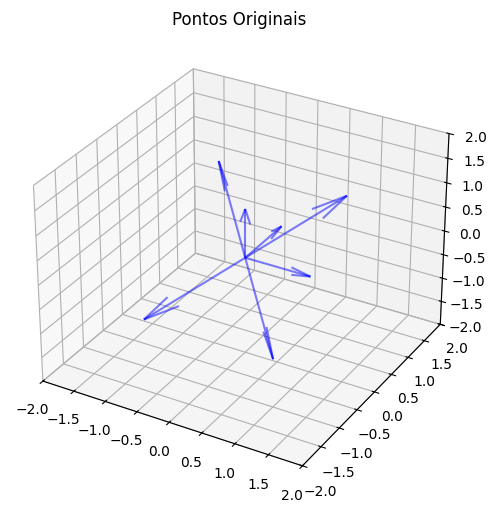
\includegraphics[width=0.75\linewidth]{image9.png}
\end{figure}
\begin{figure}
    \centering
    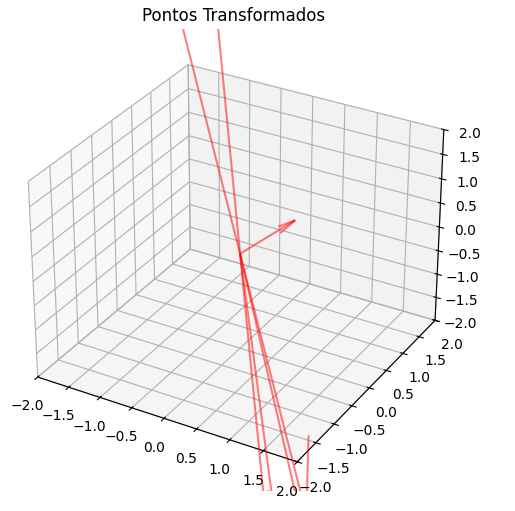
\includegraphics[width=0.75\linewidth]{image10.png}
\end{figure}
=
=============================================================================================
=
\textbf{3- Considere a forma quadrática f(x,y)=a x2 +b y2 + c xy onde a, e c são os últimos algarismos do seu RA . a) Analise o comportamento desta função no entorno da origem (0,0) , usando a diagonalização da matriz associada. b) Analise e exemplifique as cônicas que são dadas pelas curvas de nível f(x,y) = k para três diferentes valores de k ( k>0 , k =0 e k <0).}

A- A forma quadrática \( f(x, y) = 8x^2 + 2y^2 + 3xy \) pode ser representada pela matriz simétrica:
\[
A = \begin{pmatrix}
8 & \frac{3}{2} \\
\frac{3}{2} & 2
\end{pmatrix}
\]
Encontrar os autovalores:
-
A equação característica é dada por:
\[
\det(A - \lambda I) = 0
\]
onde \(I\) é a matriz identidade. 
\[
\det \begin{pmatrix}
8 - \lambda & \frac{3}{2} \\
\frac{3}{2} & 2 - \lambda
\end{pmatrix} = (8 - \lambda)(2 - \lambda) - \left(\frac{3}{2}\right)^2 = 0
\]
Simplificando, obtemos a equação característica:
\[
(8 - \lambda)(2 - \lambda) - \frac{9}{4} = 0
\]
\[
16 - 10\lambda + \lambda^2 - \frac{9}{4} = 0
\]
\[
4\lambda^2 - 40\lambda + 64 - 9 = 0
\]
\[
4\lambda^2 - 40\lambda + 55 = 0
\]
 \(\lambda\):
\[
\lambda = \frac{40 \pm \sqrt{1600 - 880}}{8} = \frac{40 \pm \sqrt{720}}{8} = \frac{40 \pm 6\sqrt{5}}{8} = 5 \pm \frac{3\sqrt{5}}{2}
\]
Os autovalores são:
\[
\lambda_1 = 5 + \frac{3\sqrt{5}}{2}, \quad \lambda_2 = 5 - \frac{3\sqrt{5}}{2}
\]
Encontrar os autovetores:
Para \(\lambda_1 = 5 + \frac{3\sqrt{5}}{2}\):
\[
\begin{pmatrix}
8 - \left(5 + \frac{3\sqrt{5}}{2}\right) & \frac{3}{2} \\
\frac{3}{2} & 2 - \left(5 + \frac{3\sqrt{5}}{2}\right)
\end{pmatrix}
\begin{pmatrix}
x \\
y
\end{pmatrix} = 0
\]
Para \(\lambda_2 = 5 - \frac{3\sqrt{5}}{2}\):
\[
\begin{pmatrix}
8 - \left(5 - \frac{3\sqrt{5}}{2}\right) & \frac{3}{2} \\
\frac{3}{2} & 2 - \left(5 - \frac{3\sqrt{5}}{2}\right)
\end{pmatrix}
\begin{pmatrix}
x \\
y
\end{pmatrix} = 0
\]
Os autovetores correspondentes são encontrados resolvendo os sistemas lineares.

B- Para \( k > 0 \):
   A equação \( f(x, y) = k \) representa uma elipse se \( a \cdot b > \left( \frac{c}{2} \right)^2 \). No nosso caso:
   \[
   8 \cdot 2 > \left( \frac{3}{2} \right)^2
   \]
\[
   16 > \frac{9}{4}
\]
   Então, para \( k > 0 \), a curva de nível é uma elipse.
-
Para \( k = 0 \):
   A equação \( f(x, y) = 0 \) representa duas retas passando pela origem.
-
Para \( k < 0 \):
   A equação \( f(x, y) = k \) representa uma hipérbole.

Código Python para Visualizar as Cônicas
-
import numpy as np
import matplotlib.pyplot as plt
from matplotlib.patches import Ellipse

# Coeficientes da forma quadrática
a = 8
b = 2
c = 3

# Função para plotar cônicas
def plot_conics(a, b, c, k_values):
    x = np.linspace(-10, 10, 400)
    y = np.linspace(-10, 10, 400)
    X, Y = np.meshgrid(x, y)
    F = a * X**2 + b * Y**2 + c * X * Y

    fig, ax = plt.subplots(1, len(k_values), figsize=(18, 6))

    for i, k in enumerate(k_values):
        ax[i].contour(X, Y, F, levels=[k], colors='blue')
        ax[i].set_title(f'f(x, y) = {k}')
        ax[i].set_xlim([-10, 10])
        ax[i].set_ylim([-10, 10])
        ax[i].axhline(0, color='black',linewidth=0.5)
        ax[i].axvline(0, color='black',linewidth=0.5)
        ax[i].grid(color='gray', linestyle='--', linewidth=0.5)
        ax[i].set_aspect('equal', adjustable='box')

    plt.show()

# Valores de k
k_values = [10, 0, -10]

# Plotar as cônicas
plot_conics(a, b, c, k_values)
-
\begin{figure}
    \centering
    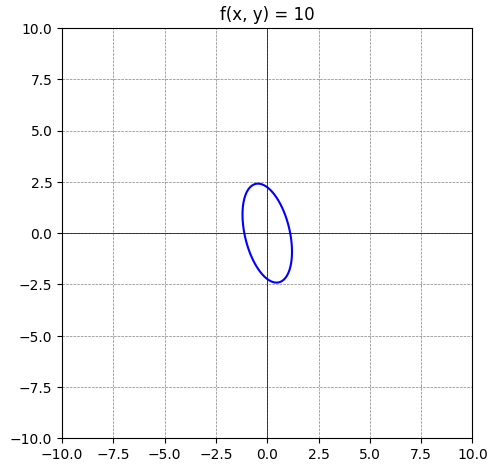
\includegraphics[width=0.75\linewidth]{image11.png}
\end{figure}
=
=============================================================================================
=
\textbf{4- Analise um outro exemplo de outra natureza de formas quadráticas em R²}
=
Vamos considerar a forma quadrática:
\[
f(x, y) = x^2 - 4y^2
\]
Análise do comportamento no entorno da origem
\[
A = \begin{pmatrix}
1 & 0 \\
0 & -4
\end{pmatrix}
\]
Como \(A\) já é uma matriz diagonal, os autovalores são os elementos da diagonal principal:
\[
\lambda_1 = 1, \quad \lambda_2 = -4
\]
Os autovetores correspondentes são simplesmente os vetores canônicos \(\begin{pmatrix} 1 \\ 0 \end{pmatrix}\) e \(\begin{pmatrix} 0 \\ 1 \end{pmatrix}\).
Os sinais dos autovalores indicam que a forma quadrática representa uma hipérbole, pois temos autovalores de sinais opostos.
Análise das curvas de nível \(f(x, y) = k\)
-
Para \(k > 0\):
   A equação \(f(x, y) = k\) representa uma hipérbole, pois temos uma diferença de quadrados que é igual a um número positivo:
   \[
   x^2 - 4y^2 = k
   \]
-
Para \(k = 0\):
   A equação \(f(x, y) = 0\) representa duas retas que se cruzam na origem:
   \[
   x^2 - 4y^2 = 0 \implies x^2 = 4y^2 \implies x = \pm 2y
   \]
=
Para \(k < 0\):
   A equação \(f(x, y) = k\) também representa uma hipérbole, mas com orientação diferente:
   \[
   x^2 - 4y^2 = k
   \]

Código Python para Visualizar as Curvas de Nível

import numpy as np
import matplotlib.pyplot as plt

# Coeficientes da forma quadrática
a = 1
b = -4
c = 0

# Função para plotar cônicas
def plot_conics(a, b, c, k_values):
    x = np.linspace(-10, 10, 400)
    y = np.linspace(-10, 10, 400)
    X, Y = np.meshgrid(x, y)
    F = a * X**2 + b * Y**2 + c * X * Y

    fig, ax = plt.subplots(1, len(k_values), figsize=(18, 6))

    for i, k in enumerate(k_values):
        ax[i].contour(X, Y, F, levels=[k], colors='blue')
        ax[i].set_title(f'f(x, y) = {k}')
        ax[i].set_xlim([-10, 10])
        ax[i].set_ylim([-10, 10])
        ax[i].axhline(0, color='black',linewidth=0.5)
        ax[i].axvline(0, color='black',linewidth=0.5)
        ax[i].grid(color='gray', linestyle='--', linewidth=0.5)
        ax[i].set_aspect('equal', adjustable='box')

    plt.show()

# Valores de k
k_values = [10, 0, -10]

# Plotar as cônicas
plot_conics(a, b, c, k_values)


Este código deve gerar gráficos das curvas de nível para \(k = 10\), \(k = 0\) e \(k = -10\). 
\begin{figure}
    \centering
    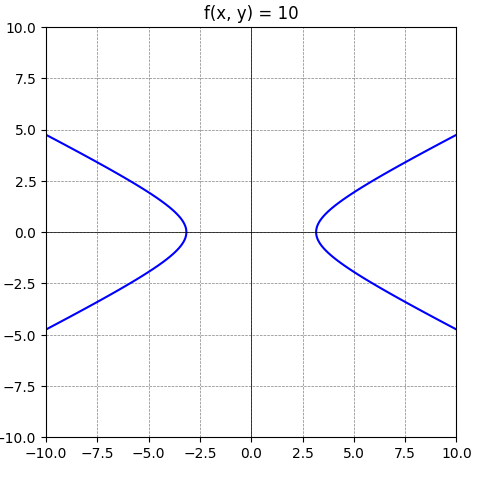
\includegraphics[width=0.75\linewidth]{image12.png}
\end{figure}
\begin{figure}
    \centering
    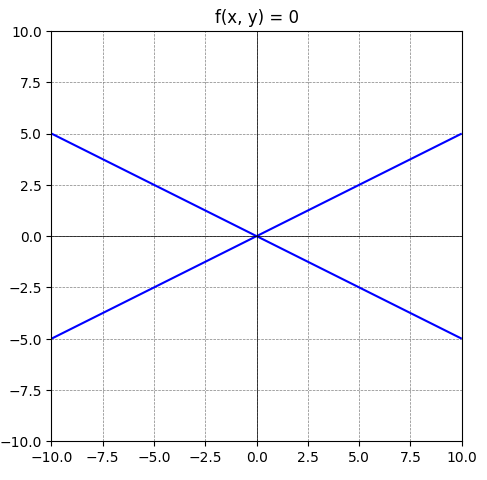
\includegraphics[width=0.75\linewidth]{image13.png}
\end{figure}
\begin{figure}
    \centering
    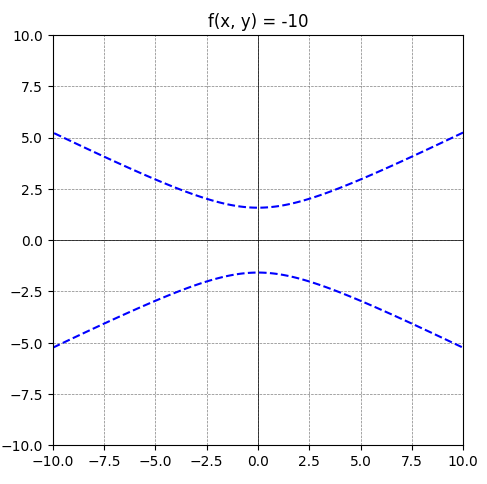
\includegraphics[width=0.75\linewidth]{image14.png}
\end{figure}
- Para \(k > 0\), obtemos hipérboles que abrem para os lados.
- Para \(k = 0\), obtemos duas retas que se cruzam na origem.
- Para \(k < 0\), obtemos hipérboles que abrem para cima e para baixo.
=
==============================================================================================

\[
f(x, y, z) = 0x^2 + 3y^2 + 7z^2 + 3xy + 8xz + 2yz
\]
\[
A =\begin{pmatrix}
0 & \frac{3}{2} & 4 \\
\frac{3}{2} & 3 & 1 \\
4 & 1 & 7
\end{pmatrix}
\]
\( A - \lambda I \):
\[
\begin{pmatrix}
0 - \lambda & \frac{3}{2} & 4 \\
\frac{3}{2} & 3 - \lambda & 1 \\
4 & 1 & 7 - \lambda
\end{pmatrix}
\]

Determinante:
\[
\det \begin{pmatrix}
-\lambda & \frac{3}{2} & 4 \\
\frac{3}{2} & 3 - \lambda & 1 \\
4 & 1 & 7 - \lambda
\end{pmatrix} = 0
\]

Vamos expandir o determinante:
\[
-\lambda \left| \begin{array}{cc}
3 - \lambda & 1 \\
1 & 7 - \lambda
\end{array} \right| - \frac{3}{2} \left| \begin{array}{cc}
\frac{3}{2} & 4 \\
1 & 7 - \lambda
\end{array} \right| + 4 \left| \begin{array}{cc}
\frac{3}{2} & 3 - \lambda \\
1 & 1
\end{array} \right|
\]

Calculando os determinantes menores:
\[
\left| \begin{array}{cc}
3 - \lambda & 1 \\
1 & 7 - \lambda
\end{array} \right| = (3 - \lambda)(7 - \lambda) - 1 = 21 - 10\lambda + \lambda^2 - 1 = \lambda^2 - 10\lambda + 20
\]

\[
\left| \begin{array}{cc}
\frac{3}{2} & 4 \\
1 & 7 - \lambda
\end{array} \right| = \frac{3}{2}(7 - \lambda) - 4 = \frac{21 - 3\lambda - 8}{2} = \frac{13 - 3\lambda}{2}
\]

\[
\left| \begin{array}{cc}
\frac{3}{2} & 3 - \lambda \\
1 & 1
\end{array} \right| = \frac{3}{2}(1) - (3 - \lambda) = \frac{3}{2} - 3 + \lambda = \lambda - \frac{3}{2}
\]

A equação característica se torna:
\[
-\lambda (\lambda^2 - 10\lambda + 20) - \frac{3}{2} \left( \frac{13 - 3\lambda}{2} \right) + 4 (\lambda - \frac{3}{2}) = 0
\]
\[
-\lambda^3 + 10\lambda^2 - 20\lambda - \frac{39 - 9\lambda}{4} + 4\lambda - 6 = 0
\]
\[
-\lambda^3 + 10\lambda^2 - 20\lambda + 6.25\lambda - 9.75 = 0
\]
\[
-\lambda^3 + 10\lambda^2 - 13.75\lambda - 9.75 = 0
\]

B: Superfície de nível \( f(x, y, z) = k \)
-
Para \( k = 1 \), temos:
\[
0x^2 + 3y^2 + 7z^2 + 3xy + 8xz + 2yz = 1
\]
-
Código Python para Visualizar a Superfície de Nível

import numpy as np
import matplotlib.pyplot as plt
from mpl_toolkits.mplot3d import Axes3D

# Definindo a função f(x, y, z)
def f(x, y, z):
    return 3*y**2 + 7*z**2 + 3*x*y + 8*x*z + 2*y*z

# Geração dos pontos
x = np.linspace(-10, 10, 400)
y = np.linspace(-10, 10, 400)
z = np.linspace(-10, 10, 400)

X, Y, Z = np.meshgrid(x, y, z)
F = f(X, Y, Z)

# Plotar a superfície de nível f(x, y, z) = k
fig = plt.figure(figsize=(10, 8))
ax = fig.add_subplot(111, projection='3d')
ax.contour3D(X, Y, Z, F, levels=[1], cmap='viridis')
ax.set_xlabel('X axis')
ax.set_ylabel('Y axis')
ax.set_zlabel('Z axis')
ax.set_title('Superfície de Nível f(x, y, z) = 1')

plt.show()


Este código deve gerar uma visualização 3D da superfície de nível \( f(x, y, z) = 1 \). 
\begin{figure}
    \centering
    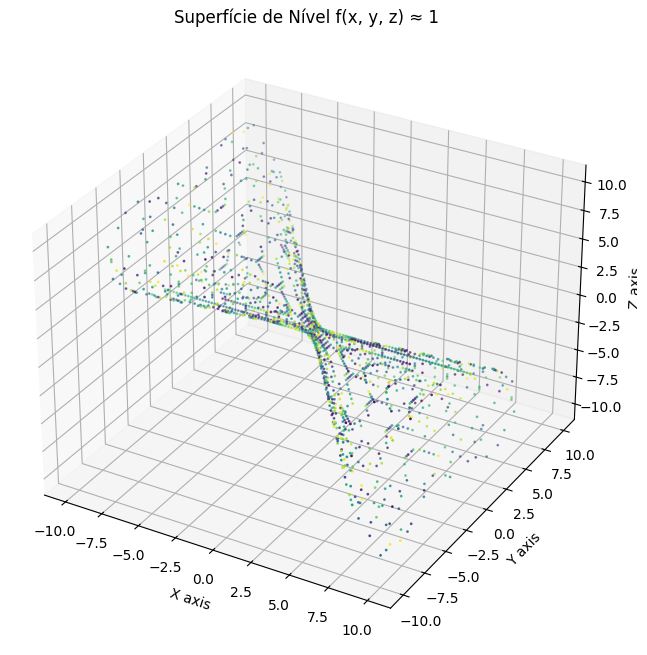
\includegraphics[width=0.75\linewidth]{image15.png}
\end{figure}
=
==============================================================================================
\textbf{6- Escolha para resolver um problema interessante de aplicação referente ao conteúdo dos Capítulos 6 a 11 do livro ( não abordado na Atividade 3).}
Para criar uma demonstração de aplicações da análise de formas quadráticas ao estudo de vibrações, podemos focar na análise modal de um sistema mecânico simples, como um sistema massa-mola. 
-
Definição do Sistema
-
Considere um sistema massa-mola com duas massas \(m_1\) e \(m_2\) conectadas por três molas com constantes \(k_1\), \(k_2\) e \(k_3\).
Formação da Matriz de Rigidez e Matriz de Massa
As equações do movimento para o sistema massa-mola são:
\[
m_1 \ddot{x}_1 + k_1 x_1 - k_2 (x_2 - x_1) = 0
\]
\[
m_2 \ddot{x}_2 + k_3 x_2 - k_2 (x_2 - x_1) = 0
\]
Podemos escrever isso na forma matricial:
\[
M \ddot{\mathbf{x}} + K \mathbf{x} = 0
\]
onde
\[
\mathbf{x} = \begin{pmatrix} x_1 \\ x_2 \end{pmatrix}
\]
A matriz de massa \(M\) e a matriz de rigidez \(K\) são:
\[
M = \begin{pmatrix} m_1 & 0 \\ 0 & m_2 \end{pmatrix}
\]
\[
K = \begin{pmatrix} k_1 + k_2 & -k_2 \\ -k_2 & k_2 + k_3 \end{pmatrix}
\]
Formação da Equação de Movimento
Para encontrar as frequências naturais e modos de vibração, buscamos soluções do tipo harmônico:
\[
\mathbf{x}(t) = \mathbf{X} e^{i\omega t}
\]
Substituindo na equação de movimento, obtemos:
\[
-\omega^2 M \mathbf{X} + K \mathbf{X} = 0
\]
Esta é uma equação de autovalores da forma:
\[
(K - \omega^2 M) \mathbf{X} = 0
\]
Análise Modal via Diagonalização
-
Para resolver esta equação, diagonalizamos o problema buscando os autovalores \(\omega^2\) e autovetores \(\mathbf{X}\). Os autovalores são as frequências naturais ao quadrado, e os autovetores são os modos de vibração.
Exemplo Numérico
Considere \(m_1 = m_2 = 1\) kg, \(k_1 = k_2 = k_3 = 1\) N/m.
A matriz de rigidez e a matriz de massa são:
\[
M = \begin{pmatrix} 1 & 0 \\ 0 & 1 \end{pmatrix}, \quad K = \begin{pmatrix} 2 & -1 \\ -1 & 2 \end{pmatrix}
\]
A equação característica é:
\[
\det(K - \omega^2 M) = \det \begin{pmatrix} 2 - \omega^2 & -1 \\ -1 & 2 - \omega^2 \end{pmatrix} = 0
\]
Calculamos o determinante:
\[
(2 - \omega^2)^2 - (-1)^2 = 0
\]
\[
(2 - \omega^2)^2 - 1 = 0
\]
\[
(2 - \omega^2 - 1)(2 - \omega^2 + 1) = 0
\]
\[
\omega^2 - 3 = 0 \quad \text{ou} \quad \omega^2 - 1 = 0
\]
\[
\omega^2 = 3 \quad \text{ou} \quad \omega^2 = 1
\]
As frequências naturais são \(\omega_1 = \sqrt{3}\) rad/s e \(\omega_2 = 1\) rad/s.
-
Interpretação Física dos Resultados

Os autovetores correspondentes aos autovalores nos dão os modos de vibração. Solucionando para \(\omega^2 = 3\) e \(\omega^2 = 1\):

Para \(\omega^2 = 3\):
\[
(K - 3M) \mathbf{X} = 0 \implies \begin{pmatrix} 2 - 3 & -1 \\ -1 & 2 - 3 \end{pmatrix} \begin{pmatrix} X_1 \\ X_2 \end{pmatrix} = 0 \implies \begin{pmatrix} -1 & -1 \\ -1 & -1 \end{pmatrix} \begin{pmatrix} X_1 \\ X_2 \end{pmatrix} = 0
\]
\[
X_1 = -X_2
\]

Para \(\omega^2 = 1\):
\[
(K - 1M) \mathbf{X} = 0 \implies \begin{pmatrix} 2 - 1 & -1 \\ -1 & 2 - 1 \end{pmatrix} \begin{pmatrix} X_1 \\ X_2 \end{pmatrix} = 0 \implies \begin{pmatrix} 1 & -1 \\ -1 & 1 \end{pmatrix} \begin{pmatrix} X_1 \\ X_2 \end{pmatrix} = 0
\]
\[
X_1 = X_2
\]
Visualizar essas frequências naturais e modos de vibração usando Python.

import numpy as np
import matplotlib.pyplot as plt
# Parâmetros do sistema
m1 = 1
m2 = 1
k1 = 1
k2 = 1
k3 = 1

# Matrizes
M = np.array([[m1, 0], [0, m2]])
K = np.array([[k1 + k2, -k2], [-k2, k2 + k3]])
# Solução do problema de autovalores
eigvals, eigvecs = np.linalg.eig(np.linalg.inv(M).dot(K))
# Frequências naturais
omega = np.sqrt(eigvals)
# Modos de vibração
modes = eigvecs
# Plotar os modos de vibração
fig, ax = plt.subplots(1, 2, figsize=(14, 6))
x = np.linspace(0, 2, 100)
for i in range(2):
    y = np.sin(omega[i] * x)
    ax[i].plot(x, y, label=f'Modo {i+1}: ω = {omega[i]:.2f} rad/s')
    ax[i].set_title(f'Modo de Vibração {i+1}')
    ax[i].set_xlabel('Tempo (s)')
    ax[i].set_ylabel('Deslocamento')
    ax[i].legend()
    ax[i].grid(True)
plt.show()
=
=
Definição das Matrizes de Massa e Rigidez: parâmetros fornecidos para definir as matrizes.
Solução do Problema de Autovalores: Usamos `np.linalg.eig` para encontrar as frequências naturais e modos de vibração.
Visualização dos Modos de Vibração: modos de vibração como funções do tempo.
=
\begin{figure}
    \centering
    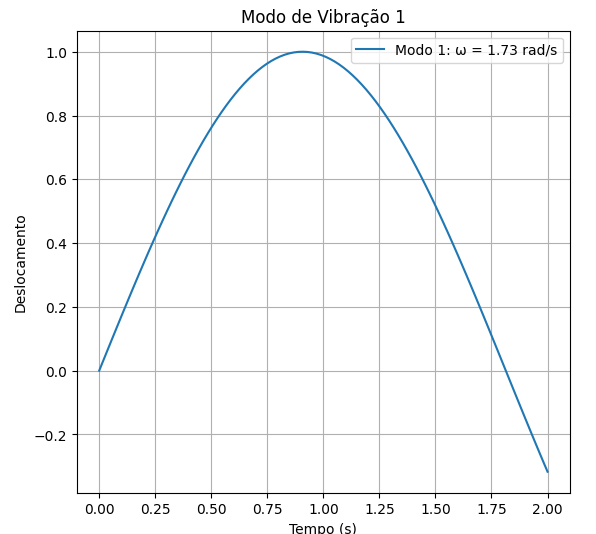
\includegraphics[width=0.75\linewidth]{image16.png}
\end{figure}
=
\begin{figure}
    \centering
    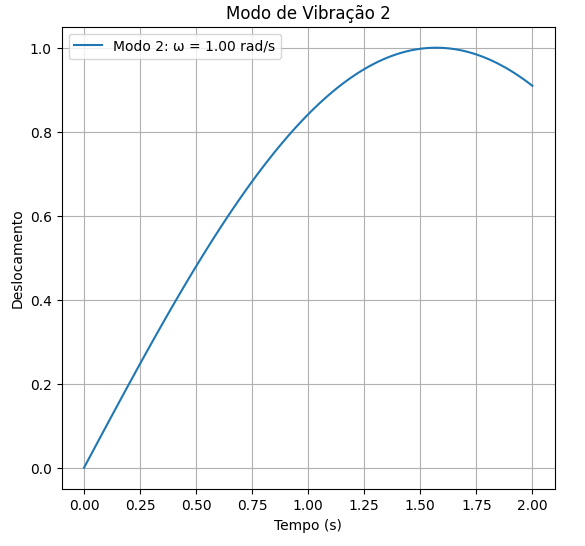
\includegraphics[width=0.75\linewidth]{image17.png}
\end{figure}
=
=============================================================================================

\end{document}
